\chapter{Introduction}

\section{Définition du Handicap}
Handicap est un mot simple qui tire son origine de l'expression "hand in the cap" (la main dans le chapeau). Cette expression désignait une transaction au cours de laquelle deux personnes, souhaitant échanger des objets de valeur différente, confiaient le r\^ole d'arbitre à un tiers. Ce dernier évaluait la somme d'argent à ajouter à l'objet de moindre valeur pour que l'échange soit équitable. La transaction se déroulait ensuite dans un chapeau dans lequel les participants plaçaient la somme qu'ils jugeaient adéquate.\\

Le mot Handicap est également appliqué à la compétition équestre. Lorsque deux chevaux de calibres différents concourraient ensemble, le meilleur était lesté d’un poids appelé « handicap » afin de maintenir l’égalité de chance entre les deux.\\

\noindent La loi de février 2005 apporte une nouvelle définition au handicap :

\begin{quotation}
\noindent Constitue un handicap, au sens de la présente loi, toute limitation d’activité ou restriction de participation à la vie en société \underline{subie dans son environnement} par une personne en raison d’une altération substantielle, durable ou définitive d’une ou plusieurs fonctions physiques, sensorielles, mentales, cognitives ou psychiques, d’un polyhandicapé ou d’un trouble de santé invalidant.\\
\end{quotation}


Le schéma de Wood (Figure \ref{schema_wood}) présente une définition du handicap, qui est d'ailleurs beaucoup utilisée dans les livres traitants du handicap. Il se base sur le fait que le handicap part de la base d'une \textbf{Déficience} (une hémiplégie ou une paralysie du membre supérieur par exemple). Cette déficience va ensuite entraîner une \textbf{Incapacité} de la personne handicapée (par exemple, l'incapacité de marcher ou l'incapacité de tenir un objet). Enfin, cette incapacité donnera lieu à un handicap. Le handicap est ainsi défini comme un désavantage social qui résultera au fait que la personne handicapée ne pourra pas reprendre d'activités professionnelles.\\
Cependant, le modèle de Wood est incomplet car certains cas particuliers ne peuvent pas être pris en compte. Par exemple, une personne ayant une brûlure du visage possède une déficience et un désavantage social, mais pas forcément une incapacité.\\

\begin{figure}
\label{schema_wood}
\centering
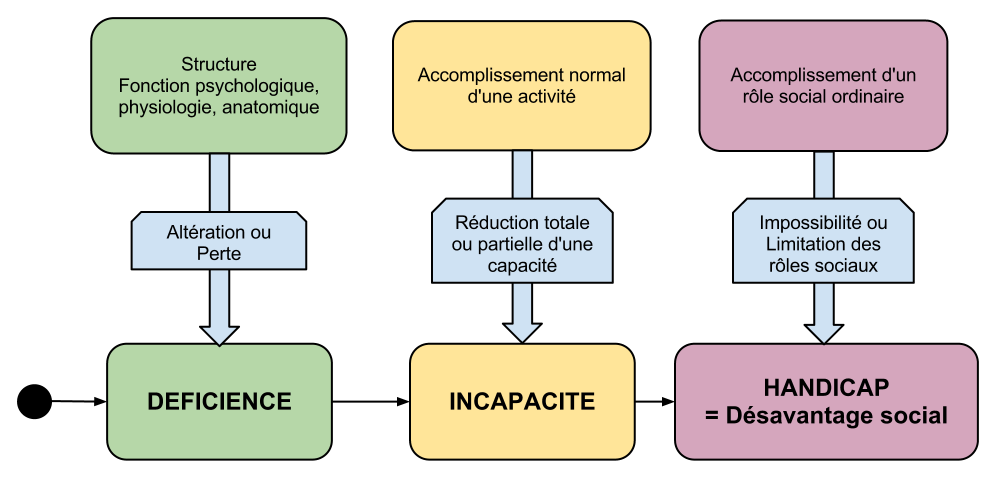
\includegraphics[scale=0.45]{figures/schema_wood.png}
\caption{Définition du Handicap selon le schéma de Wood}
\end{figure}

C'est pourquoi, pour définir le handicap, il est alors préférable de se baser sur le modèles du canadien Fougeyrollas dans les "Processus de Production du Handicap" (Figure \ref{modele_canadien}). Ce modèle prend en compte la dimension culturelle et environnementale d'une personne handicapée, ce que ne faisait pas le schéma de Wood.

\begin{figure}[H]
\label{modele_canadien}
\centering
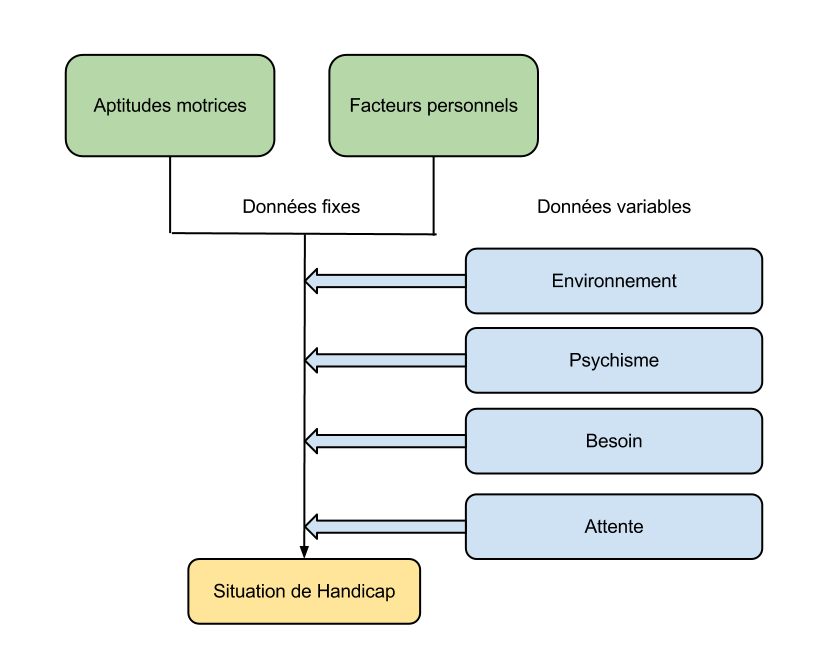
\includegraphics[scale=0.45]{figures/modele_canadien.png}
\caption{Définition du Handicap selon le modèle du canadien Fougeyrollas}
\end{figure}

La situation d'handicap part d'une base fixe constitué des aptitudes motrices de la personne handicapée et de ses facteurs personnels (identité personnelle et socio-culturelle, âge, sexe, déficiences, capacités/incapacités). 

La situation d'handicap va ensuite être modifiée par une dimension culturelle et environnementale, composée de :
\begin{itemize}
\item Les facteurs environnementaux
\item Les besoins de la personne handicapée
\item Les attentes de la personne handicapée
\item Le psychisme de la personne\\
\end{itemize}


En conclusion, une personne handicapée a ses aptitudes et ses capacités propres, mais la présence d'un environnement plus ou moins viable, les habitudes de vie et les attentes vont influencer sa situation d'handicap.
On peut ainsi dire que le handicap n'est pas un statut mais un \textbf{processus dynamique}. 



\section{Importance des dispositifs législatifs}
Deux lois importantes ont vu le jour au cours de ces 25 dernières années : la loi de 1987 sur l'obligation d'emploi de 6\% de travailleurs handicapées et la loi de 2005.\\

La loi du 10 juillet 1987 oblige les entreprises de 20 salariés et plus à employer 6 \% de personnes handicapées au sein de leurs équipes. Cette loi a permis la création de l'AGEFIPH (Association de Gestion du Fonds pour l'Insertion Professionnelle des Personnes Handicapées) qui récolte des pénalités appelées "contributions", versées par les entreprises ne respectant pas ce quota.\\

La loi du 11 février 2005 augmente la contribution versée en cas de non-respect du quota. Elle renforce également l'égalité des personnes handicapées sur le monde du travail : adaptation technique de poste, formation, accompagnement et aménagement des horaires.\\

Pour une entreprise, lorsque le quota n'est pas respecté, plusieurs cas de figures se présentent :
\begin{itemize}
\item Si l'entreprise possède de 20 à 199 salariés : elle doit alors verser une contribution de 400x le SMIC horaire par bénéficiaire manquant.
\item Si l'entreprise possède plus de 750 salariés : elle doit reverser une contribution de 600x le SMIC horaire par bénéficiaire manquant.
\item Si aucune action n'a été entrepris par l'entreprise dans un délai de 3 ans et qu'aucun salarié n'est un travailleur handicapé, alors l'entreprise doit reverser une contribution de 1500x le SMIC horaire par bénéficiaire manquant (et quelque soit la taille de l'entreprise).\\
\end{itemize}

Ce dernier type d'entreprise est appelé "EQZ" ou "Établissements à Quota Zéro". Ces entreprises ne réalisent aucune action en faveur de l'emploi de personnes handicapées. En septembre 2011, il y aurait 8654 entreprises à Quota Zéro en France, ce qui représenterait une proportion de 19\% au niveau national.

\section{Contexte et Problématique}
C'est dans le contexte des entreprises à quota zéro et des entreprises employant moins de 6 \% de personnes handicapées que je souhaiterai inscrire mon Projet Personnel des Humanités.\\

Durant cette 4e année à l'INSA, j'ai décidé de faire parti de l'association HandiManagement dont le but est de sensibiliser les étudiants sur le campus de l'INSA à l'insertion professionnelle des personnes handicapées et plus généralement au handicap. Les activités de cette association pendant l'année sont séparées en deux phases :
\begin{enumerate}
\item La première phase est appelée l'\textbf{acculturation}. C'est une phase où il nous est proposé de rencontrer des personnes issues du milieu du handicap (associations, personnes effectivement en situation de handicap, responsable de mission au sein des entreprises, etc.). La mission de cette phase est de nous apporter les connaissances nécessaires à la compréhension du dispositifs pour les personnes handicapées en France et de nous mettre en situation directe avec des personnes handicapées pour effacer tout préjugé.
\item La deuxième phase consiste en la préparation d'une semaine de sensibilisation courant mars pour les étudiants de l'INSA où notre r\^ole est de restituer la connaissance acquise, à travers des activités (quizz, pièce de thé\^atre, études de cas managériales, handisport, etc.)\\
\end{enumerate}

Durant la première phase, nous avons eu l'opportunité de rencontrer des entreprises employant plus de 6 \% de personnes handicapées. Ces entreprises avaient développé des missions handicap conséquentes pour permettre une bonne intégration et ainsi pour remplir le quota demandé par l'AGEFIPH.\\

Cependant, en 2012, près de 51 \% des entreprises (METTRE Référence) ne remplissaient toujours pas le quota demandé par l'AGEFIPH.\\
A travers ce PPH, je souhaite m'intéresser aux raisons de cette difficulté à embaucher des personnes handicapées.

Mes problématiques sont donc les suivantes :
\begin{itemize}
\item Pourquoi y a t'il encore en 2012, près d'une entreprise sur deux qui ne remplit pas ses obligations d'emploi de 6 \% des personnes handicapées en référence à la loi de février 2005 sur l'emploi ? \\
\item Comment y rémédier sur le terrain ?
\end{itemize}

